\documentclass[tikz,border=5pt]{standalone}
\usepackage[utf8]{inputenc}
\usepackage{tikz}
\usetikzlibrary{shapes.geometric, arrows.meta, positioning, shadows.blur, calc, fit, backgrounds}

% --- Professional Colors ---
\definecolor{baseGreen}{RGB}{39, 174, 96}       % Pretraining
\definecolor{mechBlue}{RGB}{64, 112, 175}       % RLHF/Mechanism
\definecolor{failRed}{RGB}{214, 69, 65}         % Internal Failure (Suppression/Miscalibration)
\definecolor{outcomePurple}{RGB}{142, 68, 173}  % Final Bad Outcome

% --- Global Style Definitions (Prevents Compile Errors) ---
\tikzset{
    % Base Block Style
    process/.style={
        rectangle, 
        rounded corners=2mm, 
        minimum width=3.8cm,      
        minimum height=1.0cm,     
        text centered, 
        text width=3.5cm,         
        font=\sffamily\footnotesize, 
        draw=gray!40,
        thick,
        blur shadow={shadow blur steps=3}
    },
    % Specific Role Styles
    stepBase/.style={process, fill=baseGreen!10, draw=baseGreen!80!black},
    stepMech/.style={process, fill=mechBlue!10, draw=mechBlue!80!black},
    stepFail/.style={process, fill=failRed!10, draw=failRed!80!black},
    stepResult/.style={process, fill=outcomePurple!10, draw=outcomePurple!80!black},
    % Arrow & Label Styles
    arrow/.style={-{Stealth}, thick, draw=gray!60, rounded corners},
    groupLabel/.style={font=\bfseries\sffamily\tiny, color=gray!70, anchor=north west}
}

\begin{document}

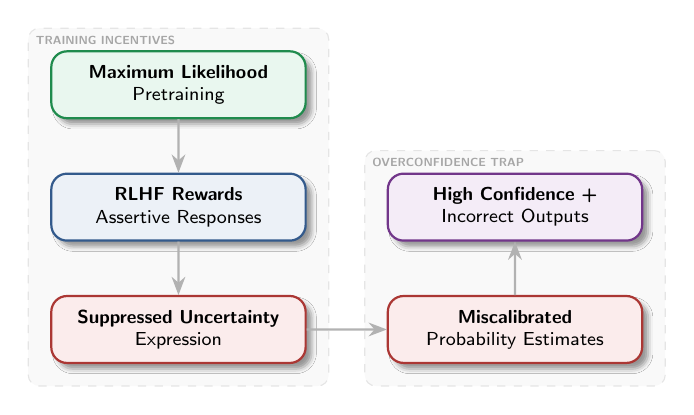
\begin{tikzpicture}[
    transform shape, 
    scale=0.85, 
    node distance=0.8cm and 1.2cm
]

    % --- LEFT COLUMN (Training Inputs) ---
    
    % 1. Pretraining
    \node (step1) [stepBase] {
        \textbf{Maximum Likelihood} \\ 
        Pretraining
    };

    % 2. RLHF
    \node (step2) [stepMech, below=of step1] {
        \textbf{RLHF Rewards} \\ 
        Assertive Responses
    };

    % 3. Suppression (Bottom Left)
    \node (step3) [stepFail, below=of step2] {
        \textbf{Suppressed Uncertainty} \\ 
        Expression
    };

    % --- RIGHT COLUMN (Calibration Failure) ---
    
    % 4. Miscalibration (Bridge to Right)
    \node (step4) [stepFail, right=of step3] {
        \textbf{Miscalibrated} \\ 
        Probability Estimates
    };

    % 5. High Confidence (Top Right)
    % Note: I placed this above step 4 to complete the U-shape
    \node (step5) [stepResult, above=of step4] {
        \textbf{High Confidence +} \\ 
        Incorrect Outputs
    };

    % --- Arrows (The U-Shape) ---
    \draw [arrow] (step1) -- (step2);
    \draw [arrow] (step2) -- (step3);
    \draw [arrow] (step3) -- (step4); % Crossing over
    \draw [arrow] (step4) -- (step5); % Moving Up

    % --- Background Grouping ---
    \begin{scope}[on background layer]
        % Group 1: Alignment Pressure
        \node [fit=(step1)(step3), fill=gray!5, draw=gray!20, rounded corners, dashed, inner sep=8pt] (groupL) {};
        \node [groupLabel] at (groupL.north west) {TRAINING INCENTIVES};
        
        % Group 2: The Calibration Gap
        \node [fit=(step4)(step5), fill=gray!5, draw=gray!20, rounded corners, dashed, inner sep=8pt] (groupR) {};
        \node [groupLabel] at (groupR.north west) {OVERCONFIDENCE TRAP};
    \end{scope}

\end{tikzpicture}
\end{document}